\documentclass{article}
\usepackage{titlesec}
\usepackage{mhchem}
\usepackage{array}
\usepackage{graphicx}
\usepackage[bmargin=2cm, tmargin=2cm]{geometry}
\usepackage{fourier-orns}

\newcommand{\thedate}[1]{\hfill{\small\sc #1}}
\newcommand{\NB}{{\large\lefthand}\quad}
\titleformat{\section}[hang]{\sc\Large}{\S\thesection}{3ex}{}[]
\titleformat{\subsection}[runin]{\sc\large}{\S\thesubsection}{3ex}{}[]
\titleformat{\subsubsection}[runin]{}{\S\thesubsubsection}{1ex}{\bfseries}[.]

\newtheorem{defn}{Definition}[section]

\begin{document}
    \section{P-block Chemistry}
    \subsection{Metalloids}
    \subsection{Electronegativity}\thedate{28/10/20 --- Week 1}
    \subsubsection{Ionisation Energy (IE)} The energy required to remove completely
    an electrion from the gaseous atom or molecule in its `ground state'.

    \begin{center}
        {\renewcommand{\arraystretch}{2}%
        \begin{tabular}[2cm]{l l}
            \ce{ M_{(g)} -> M^+_{(g)} + e-}  & First Inonisation Energy \\
            \ce{M^2+_{(g)} -> M^3+_{(g)} + e-} & Second Inonisation Energy
        \end{tabular}}
    \end{center}
        
    This process requries an input of energy (endothermic), 
    so the ionisation energy will be positive.

    Concerning the p (and s) blocks the inionisation energy increases from
    left to right (with some exceptions) and sharply decreases upon a new period. The higher (in number) the
    period the lower the ionisation energy.
    The most important factor is the distance between the nucleus and electron. With larger shells (e.g. p) the electrons
    are further away and so are not pulled on as heavily by the nucleus (lower effective nuclear charge).
    Notice on the graph where the ionisation energy does not increase across the period.
    
    \begin{figure}[h]
        \centering
        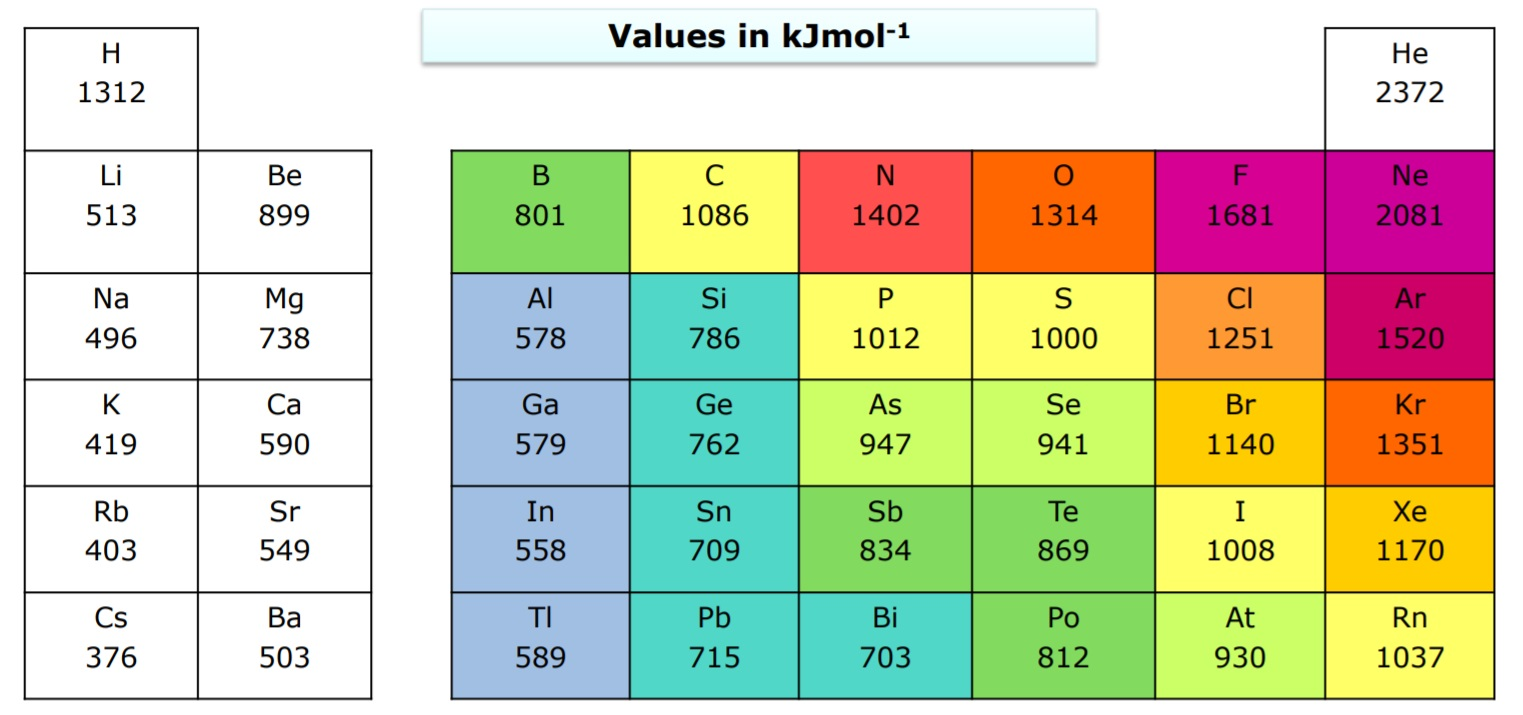
\includegraphics[width=12cm]{ionisation energy.jpg}
    \end{figure}
    \NB The ionisation energy of the metalloids are very similar (801--812), the increase in energy of going across the period
    is counteracted by moving down the table. 

    On descending groups the most irregular behaviour is seen in group 13. Ga and Ti are \emph{higher} than
    expected. Ga is preceded by the first set of d orbitals and Ti is preceded by the first set of f orbitals.
    d and f orbitals provide very weak shielding in comparison to s and p orbitals, so we have a higher effective
    nuclear charge than expected.

    \begin{figure}[h]
        \centering
        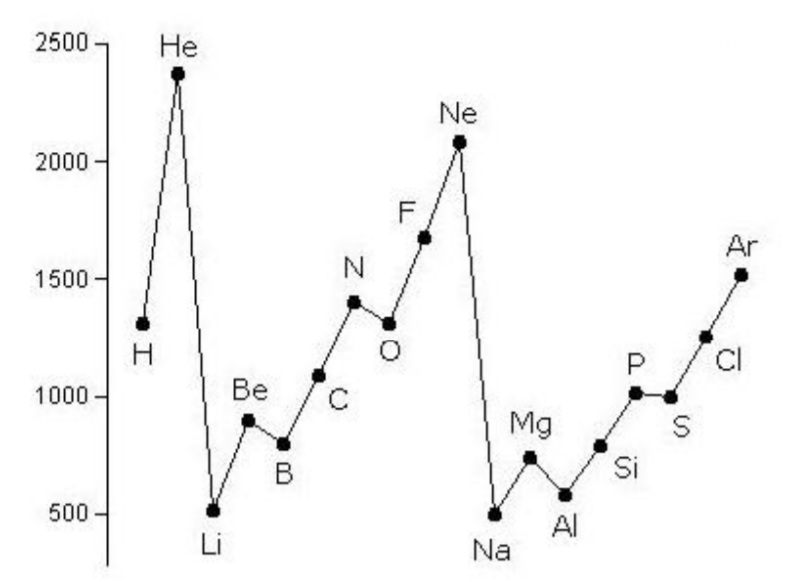
\includegraphics[width=6cm]{group13.jpg}
    \end{figure}

    The kink from Be to B comes from the Be having a full s shell, so removing an electron from Boron would be 
    favourable to give it a full s-orbital. The kink from N to O comes from Oxygen having a paired electron in its
    p-orbital, so they experience greater \emph{Coulombic repulsion}. The removal of an electron relieves this
    repulsion.

    \subsubsection{Electron Affinity (EA)} The energy release when a gaseous atom,
    molecule or ion in its `ground state' gains an electron.
    \begin{center}
        \ce{X_{(g)} + e- -> X^-_{(g)}} \hspace{4ex} First electron Affinity
    \end{center}

    Since this process is favourable and energy will be given out (exothermic),
    this electron affinity will be negative.

    \begin{figure}[h]
        \centering
        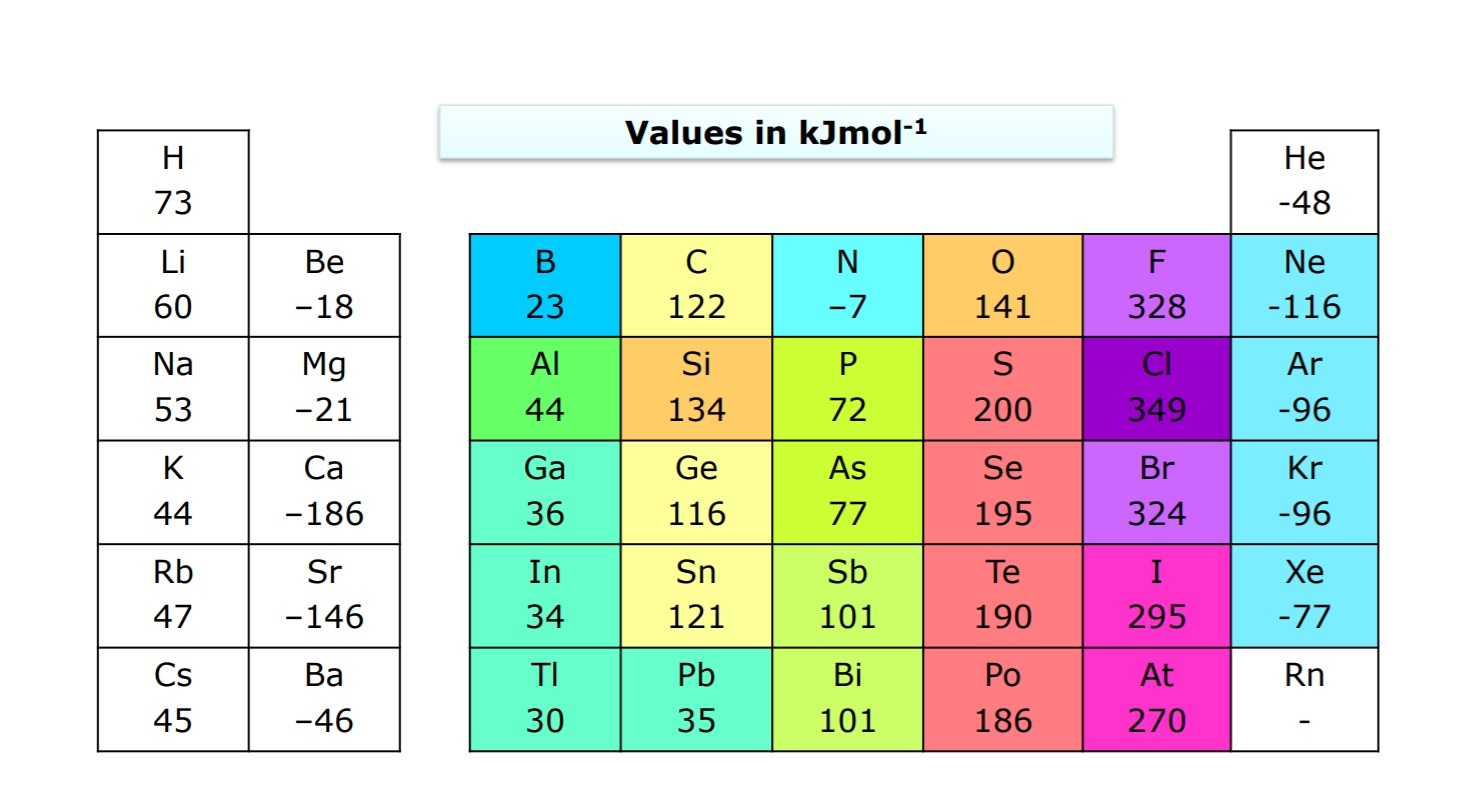
\includegraphics[width=12cm]{ea.jpg}
    \end{figure}
    \NB A positive value corresponds to energy being given out upon addition of an electron. Negative enthalpy.

    It is very unfavourable for Neon to accept an electron and break its full p orbital, and very favourable for
    Fluorine to accept an electron and fufill its shell. It generally gets smaller as you move down a group
    due to more shielding. Nitrogen's value is negative because of the energy needed to overcome the electron-
    electron repulsion that occurs when two electrons occupy the same orbital (think back to IE). 
    The same applies to all of group 15. Group 2 is also lower because it already has a full shell.
    The values of Group 13 (except for B) are all very similar due to the weak shielding provided by the 
    preceding d and f orbitals.
    The 2nd period is is smaller than the first becuase of the small size, so it has a higher charge to radius 
    ratio which gives higher repulsion.
    \begin{figure}[h]
        \centering
        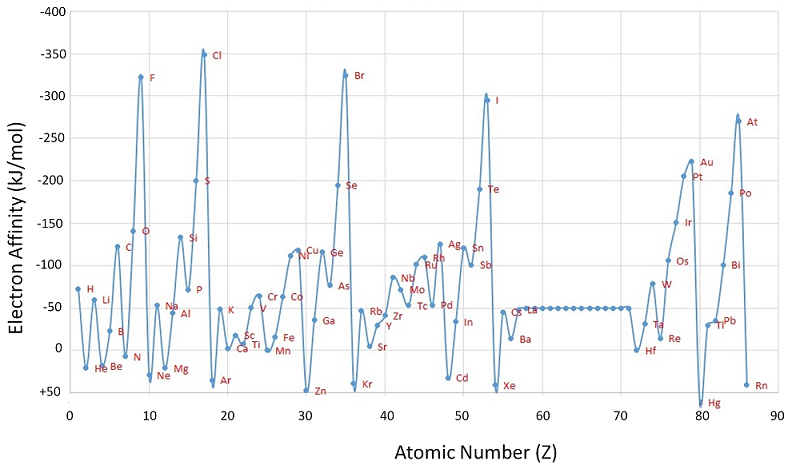
\includegraphics[width=12cm]{ea2.png}
    \end{figure}
    \newpage
    \subsubsection{Electronegativity} The ability of an atom to attract electron density towards itself in a molecule.
    
    The calculation of electronegativity using the Pauling scale.
    \begin{enumerate}
        \item A hypothetical molecule XY
        \item Compare the measured \(XY_{\text{measured}}\) bond energy with a theoretical bond energy \(XY_{\text{theoretical}}.\)
        \item \(XY_{\text{theoretical}} = \sqrt{XX^2 + YY^2}\)
        \item \(\Delta\) Bond energy = \(XY_{\text{measured}} - XY_{\text{theoretical}}\)
    \end{enumerate}

    A difference in bond energy implies a difference in electronegativity between the two atoms.
    \begin{figure}[h]
        \centering
        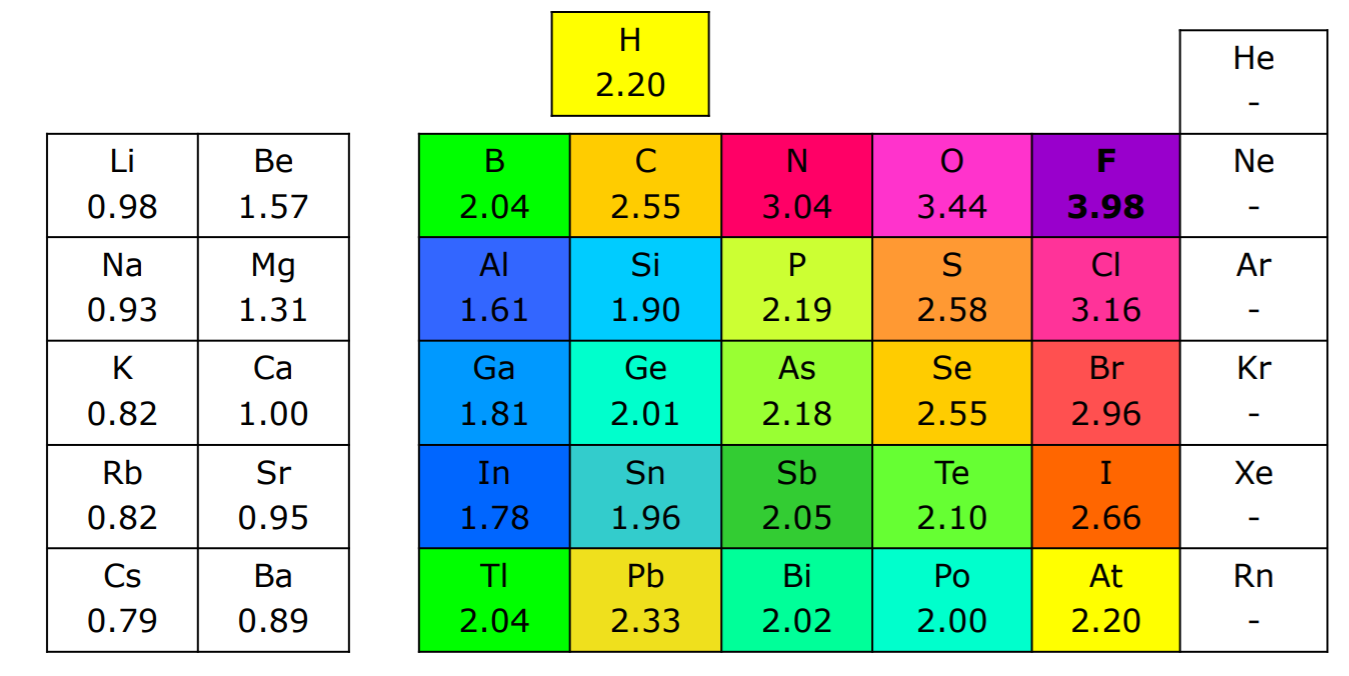
\includegraphics[width=10cm]{pauling.png}
    \end{figure}

    The electronegativity across the p-block is relatively trendy, increasing across a period and down a group,
    once again all the metalloids have a similar electronegativity. The jump in periods 4 and 5 from 3 in groups
    13 and 14 is from the d and f orbitals which provide weak shielding, giving them a higher effective nuclear 
    charge. Electronegativity varies depending on the hybridisation, sp \(>\) sp \(^2\) \(>\) sp\(^3\).
    \begin{figure}[h]
        \centering
        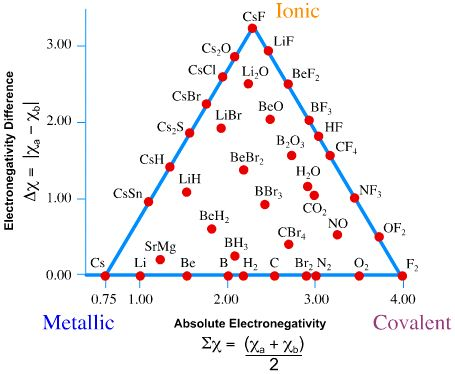
\includegraphics[width=8cm]{triangle.jpg}
    \end{figure}
    The van Arkel Ketelaar triangle is valid for simple sp compounds. 

    \subsubsection{Summary}
    \begin{itemize}
        \item Ionisation energies increase left to right and decrease top to bottom
        \item Electron affinities broadly increase left to right
        \item Electronegativity increases left to right and decreases top to bottom
    \end{itemize}
    Further reading: Inorganic Chemistry (M. Weller, T. Overton et al) (7th edition) sections 1.7 and 2.13
    \newpage

    \subsection{Effective Nuclear Charge}\thedate{28/10/20 --- Week 1}
    \subsubsection{Slater's Rules}
    There is a trendy decrease moving across each period and a trendy increase moving down each group.
    \begin{figure}[h]
        \centering
        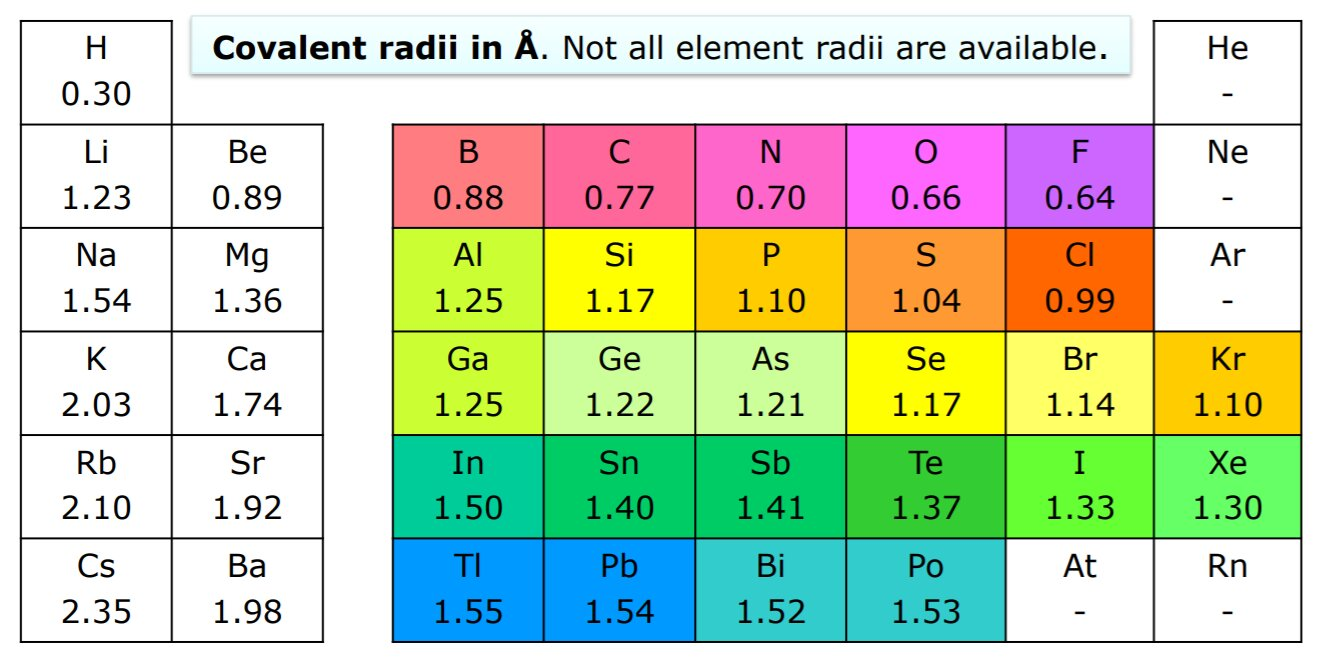
\includegraphics[width=10cm]{covrad.jpg}
        \caption{Covalent radius}
    \end{figure}

    Slater's rule: the outermost electrons `feel' a nuclear charge which is less than the actual charge because
    of shielding effects (s) from other electrons. \(Z^* = Z - s\) (\(Z^*\) is sometimes called \(Z_{\text{eff}}\))

    We can calculate the shielding constant (s) through simple calculations. 
    \begin{enumerate}
        \item Write out the electronic configuration in the following way:
        
        (1s), (2s, 2p), (3s, 3p), (3d), (4s, 4p), (4d), (4f), (5s, 5p) etc.

        \item When considering a particular electron in an ns or np orbital:
        
        Each electron with the same principal quantum number i.e. (ns, np), (nd) contributes 0.35\\
        Each electron in the (n-1) shell contributes 0.85\\
        Each electron in the (n-2) or lower shells contribute 1.00 

        \item When considering a particular electron in an nd or nf orbital:
        
        Each of the other electrins in the (nd, nf) group contributes 0.35\\
        Each of the electrons in a lower group than the one being considered contributes 1.00\\
    \end{enumerate}
    \NB Do \textbf{NOT} include the electron that you are considering when calculating \(s\), it cannot shield the
    nucleus from itself.

    \begin{figure}[h]
        \centering
        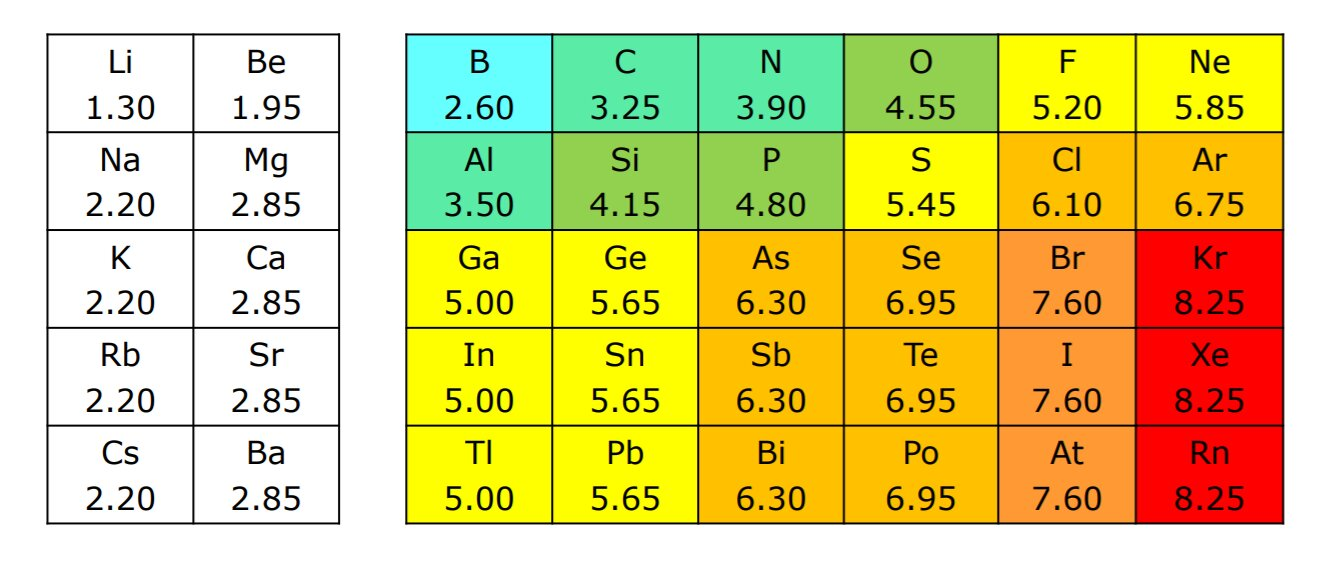
\includegraphics[width=10cm]{eff.jpg}
        \caption{Effective nuclear charge}
    \end{figure}

    The effective nuclear charge increases across a period and down a group. The values begin to flatten out at
    the bottom periods, this is because (n-2) contribtues 1.00 to s. 
    \newpage
    \begin{figure}[h]
        \centering
        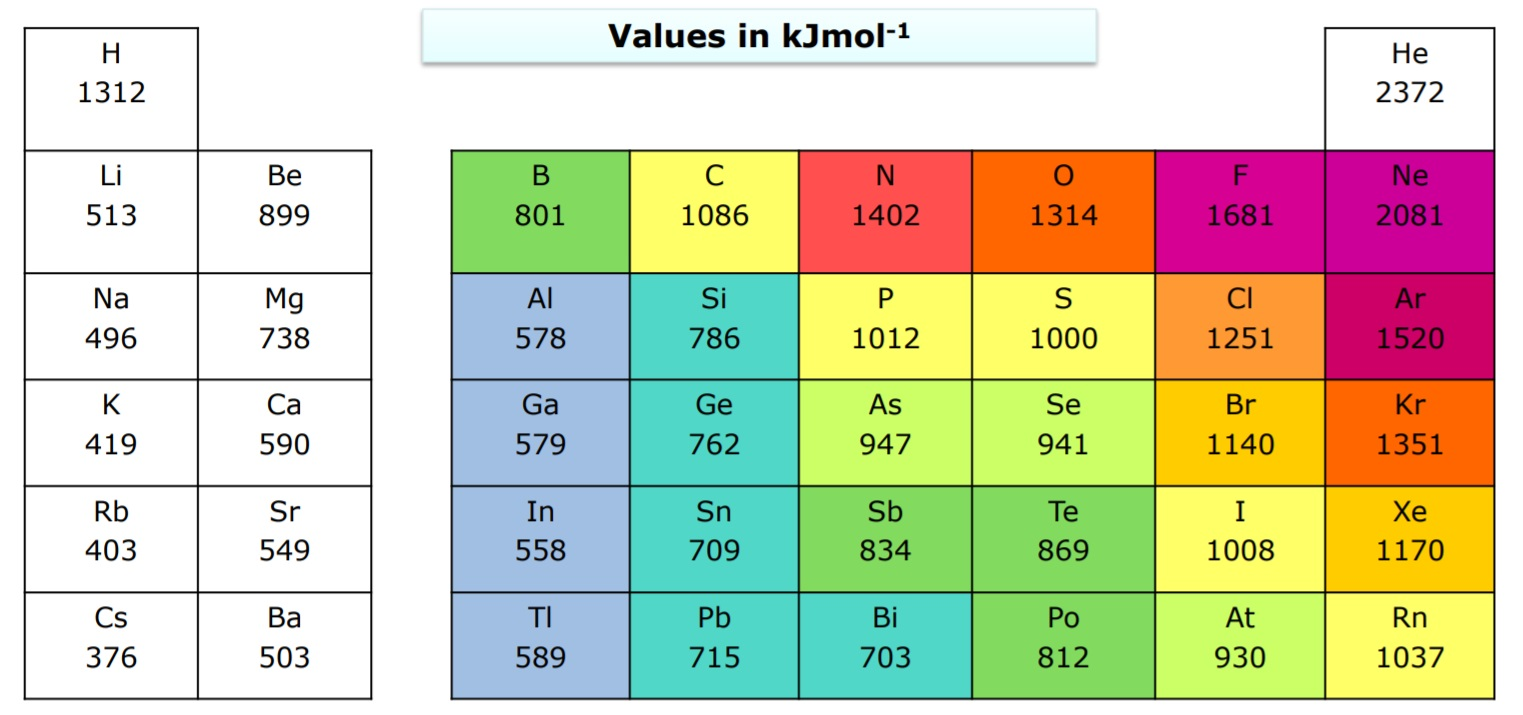
\includegraphics[width=10cm]{ionisation energy.jpg}
        \caption{Ionisation energy}
    \end{figure}

    Despite this flattening off the ionisation energy decreases down the groups (except for 13), this is because
    the radius is also an important factor for determining ionisation energy.

    \begin{figure}[h]
        \centering
        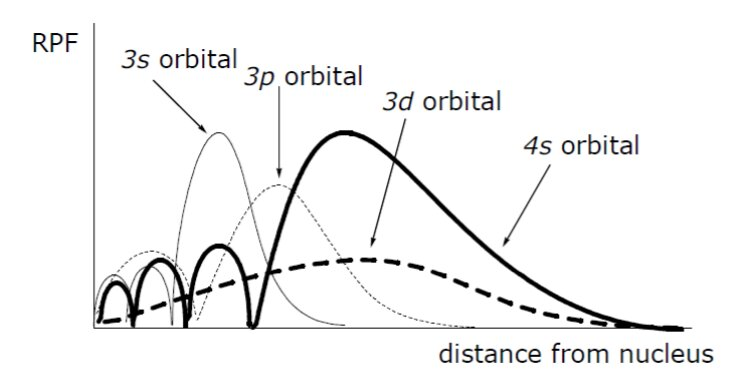
\includegraphics[width=10cm]{pen.jpg}
        \caption{RPF is the probability of finding it there}
    \end{figure}

    Slater's rules are very simplistic and can only explain the increase across period in ionisation energy, it 
    cannot explain the reduction in ionisation energy down a group. This is because it does not take into account
    the penetration of higher principal quantum number electrons. When a 4s electron is closer to the nucleus 
    it will feel more charge.
    \newpage
    \subsubsection{Covalent and Ionic Radii}

    A covalent radius is defined as half the length of a symmetrical homonuclear element bond (X-X)

    \begin{figure}[h]
        \centering
        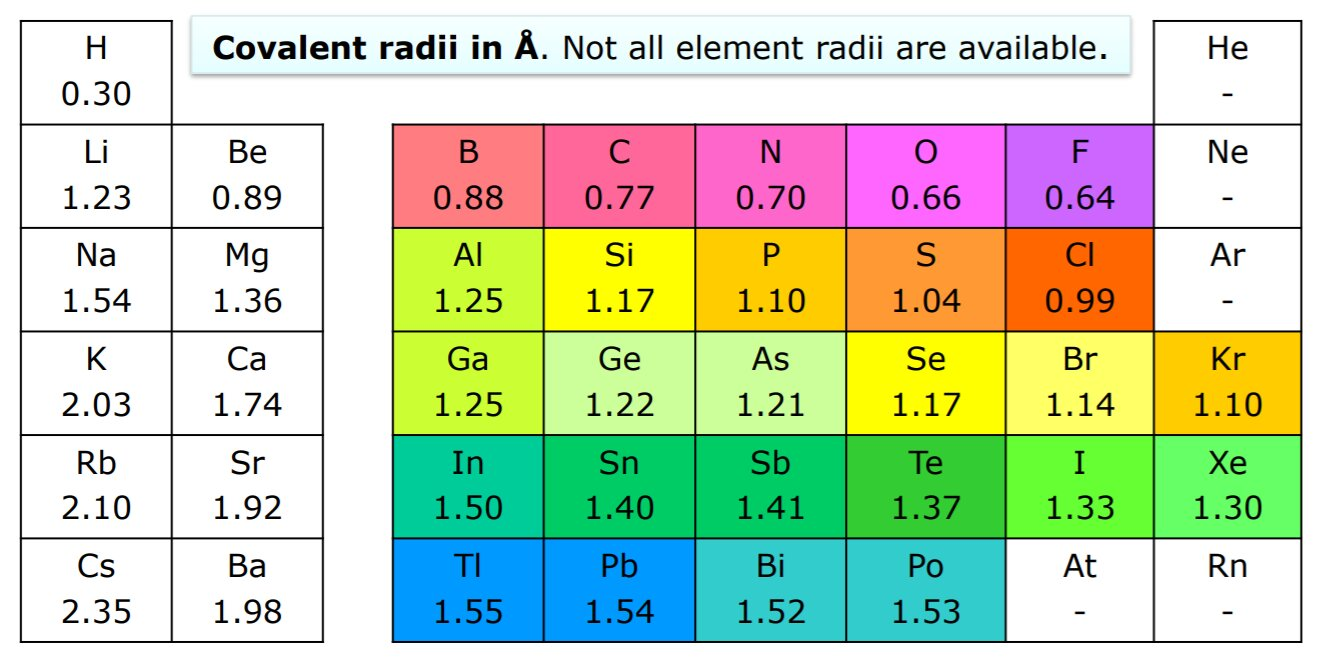
\includegraphics[width=10cm]{covrad.jpg}
        \caption{Covalent radius}
    \end{figure}

    \NB Bonds will shorten if ionic character is present, so we must account for electronegativity differences.

    Make this itemized.
    There is a decrease across a period as effective nuclear charge increases, the nuclear charge increases by 1
    whilst only decreaseing 0.35 from ony more p-electron. Radii increases down a group as the valence electrons
    are in the next principal quantum shell so they're further from the nucleus (Slater's rules cannot account
    for this). Obviously anions are large because of more inter-electron repulsion and cations are smaller because
    of a less repulsion. Thusly a higher oxidation state means a higher effective nuclear charge.
    Radii will also vary depending on the coordination number (ligands giving electron density).

    \begin{figure}[h]
        \centering
        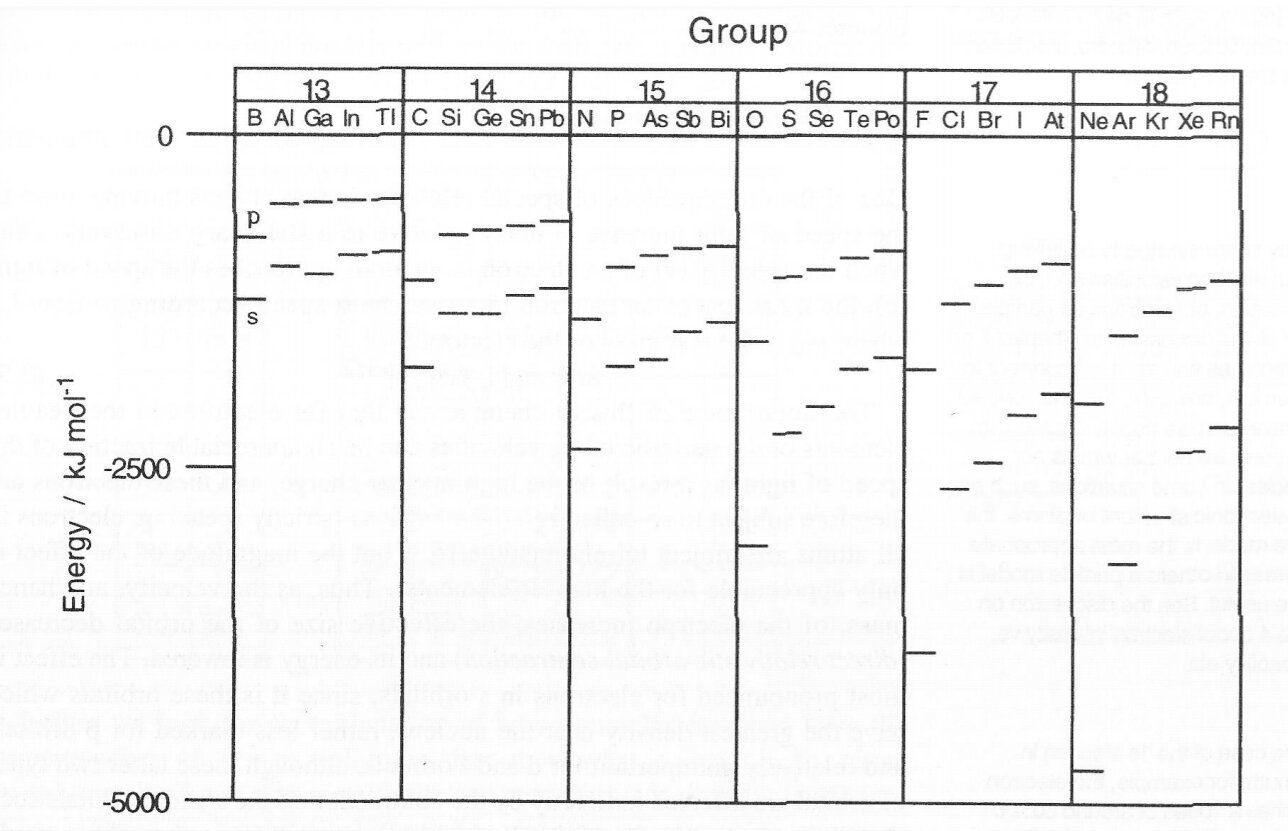
\includegraphics[width=10cm]{s-psep.jpg}
        \caption{Highest occupied orbital energies}
    \end{figure}

    Down a group the s \& p orbitals increase (less negative) in energy and the s-p energy separation decreases.
    The higher principal quantum shell electrons are further away from the nucleus and so the pull is less, giving
    a less negative energy (it's easier for the electron to leave). Ga and Ge deviate from this trend, once again
    this is from the 3d orbital preceding them, thus decreasing the energy of the s orbitals as they can penetrate
    further into the 3d orbital, making the s orbital more evenly distributed. (I don't if this is right, he said something about an s orbital being more evenly 
    distributed? \textbf{Check this out later.}) The distance between s \& p increases and the energy decreases as 
    we go across a period. Due to a better \(Z^*\) and more penetration for s. This is why the \(\sigma\) and \(\pi\)
    levels swap around from N\(_2\) to O\(_2\) (Molecular Orbitals from 1st year). The 4s orbital for As, Se, Br and
    Kr are lower than expected. This is because of the increased \(Z^*\) from their higher proton count having a strong
    effect on the 4s electrons which allow it to penetrate further into the core.  
    
    \begin{figure}[h]
        \centering
        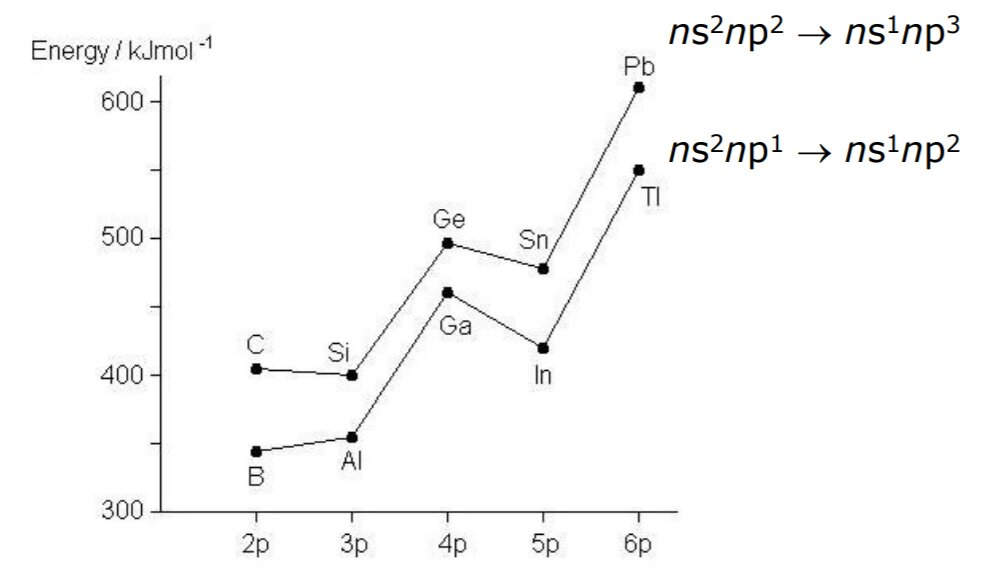
\includegraphics[width=10cm]{trans.jpg}
        \caption{Reorganisation energies of groups 13 and 14}
    \end{figure}

    As we go down a group the energy to promote an s electron to a p-orbital increases, with the sharp execption of 
    Ge and Ga, as the 4p orbital is preceded by a 3d row, so the energy of the 4p orbital is lower (more stable). 
    Unexpectedly Ti and Pb have the highest promotion energy, this has substantial implications on hybridisation
    energies. Remember when an electron moves the others do not stay static, their energies change due to
    electron correlation.

\end{document}